\PassOptionsToPackage{hidelinks}{hyperref}
\documentclass[jou]{apa7}


\begin{filecontents}{jobname.bib}
	@book{APA2014,
	title = {Manual Diagnóstico y Estadístico de Los Trastornos Mentales {{DSM-5}}},
	author = {APA, American Psychiatric Association -},
	date = {2014},
	edition = {5a. ed.},
	publisher = {Editorial Médica Panamericana},
	location = {Madrid}
  }
  
  @book{beckDepressionCausesTreatment2009,
	title = {Depression: Causes and Treatment},
	shorttitle = {Depression},
	author = {Beck, Aaron T. and Alford, Brad A.},
	date = {2009},
	edition = {2nd ed},
	publisher = {University of Pennsylvania Press},
	location = {Philadelphia},
	isbn = {978-0-8122-1964-7},
	pagetotal = {405},
	keywords = {Depression Mental,Depressive Disorder},
	annotation = {OCLC: ocn229036125}
  }
  
  @article{Bloch1983,
	title = {Enfermedades Autoinmunes. {{Patogenia}}. {{Patologia}}},
	author = {Bloch, M. and Rivera, H.},
	date = {1983},
	journaltitle = {Rev. Inst. Invest. Méd},
	pages = {248--259}
  }
  
  @article{cotaCardiometabolicRiskHealth2021,
	title = {Cardiometabolic Risk and Health Behaviours in Adolescents with Normal-Weight Obesity: A Systematic Review},
	shorttitle = {Cardiometabolic Risk and Health Behaviours in Adolescents with Normal-Weight Obesity},
	author = {Cota, Bruna Clemente and Suhett, Lara Gomes and Leite, Nathália Nogueira and Pereira, Patrícia Feliciano and Ribeiro, Sarah Aparecida Vieira and Franceschini, Sylvia Do Carmo Castro},
	date = {2021-04},
	journaltitle = {Public Health Nutrition},
	shortjournal = {Public Health Nutr.},
	volume = {24},
	number = {5},
	pages = {870--881},
	issn = {1368-9800, 1475-2727},
	doi = {10.1017/S1368980020004863},
	url = {https://www.cambridge.org/core/product/identifier/S1368980020004863/type/journal_article},
	urldate = {2024-08-03},
	abstract = {Abstract                            Objective:               To analyse the presence of cardiometabolic risk factors in adolescents with normal-weight obesity (NWO), as well as to investigate health behaviours related to the phenotype.                                         Design:               The study was conducted according to the Preferred Reporting Items for Systematic reviews and Meta-Analyses guidelines and the bibliographic search was carried out in the PubMed, Scielo and ScienceDirect databases.                                         Setting:               School, university and population.                                         Participants:               Adolescents between 10 and 19 years old.                                         Results:               A total of eight papers were included. Most studies have found a relationship between NWO and the presence of cardiometabolic risk factors, such as high waist circumference, unfavourable lipid and glycid profile. As for health behaviours, three of the eight studies included evaluated eating habits; however, the results were not conclusive. In addition, four studies analysed the practice of physical activity or physical fitness, which was lower in NWO.                                         Conclusions:               The available evidence indicates that NWO is related to the early development of cardiometabolic changes, physical inactivity and less physical fitness in adolescents. The results also reveal the importance of early detection of the phenotype, as well as the need for further research on the associated factors to prevent future diseases. Registration (PROSPERO: CRD42020161204).},
	langid = {english},
	file = {/Users/danihrndzld/Zotero/storage/39RB2UIW/Cota et al. - 2021 - Cardiometabolic risk and health behaviours in adol.pdf}
  }
  
  @article{daneshLowGradeInflammation2000,
	title = {Low Grade Inflammation and Coronary Heart Disease: Prospective Study and Updated Meta-Analyses},
	shorttitle = {Low Grade Inflammation and Coronary Heart Disease},
	author = {Danesh, J.},
	date = {2000-07-22},
	journaltitle = {BMJ},
	volume = {321},
	number = {7255},
	pages = {199--204},
	issn = {09598138},
	doi = {10.1136/bmj.321.7255.199},
	url = {https://www.bmj.com/lookup/doi/10.1136/bmj.321.7255.199},
	urldate = {2024-08-03},
	file = {/Users/danihrndzld/Zotero/storage/J6V5AEEP/Danesh - 2000 - Low grade inflammation and coronary heart disease.pdf}
  }
  
  @misc{Farlex2023,
	title = {Dictionary},
	author = {{Farlex}},
	date = {2023},
	url = {https://www.thefreedictionary.com/dictionary}
  }
  
  @article{Farre2020,
	title = {Intestinal Permeability, Inflammation and the Role of Nutrients},
	author = {Farré, R. and Fiorani, M. and Abdu Rahiman, S. and Matteoli, G.},
	date = {2020},
	journaltitle = {Nutrients},
	volume = {12},
	number = {4},
	pages = {1185},
	doi = {10.3390/nu12041185},
	file = {/Users/danihrndzld/Zotero/storage/TBS6HUGR/Farré et al. - 2020 - Intestinal permeability, inflammation and the role.pdf}
  }
  
  @inproceedings{GarciaCasal2014,
	title = {Dieta e Inflamación},
	booktitle = {Anales Venezolanos de Nutrición},
	author = {García-Casal, M. N. and Pons-Garcia, H. E.},
	date = {2014},
	volume = {27},
	number = {1},
	pages = {47--56},
	publisher = {Fundación Bengoa}
  }
  
  @article{giuglianoMetabolicCardiovascularEffects1997,
	title = {Metabolic and {{Cardiovascular Effects}} of {{Carvedilol}} and {{Atenolol}} in {{Non-Insulin-Dependent Diabetes Mellitus}} and {{Hypertension}}: {{A Randomized}}, {{Controlled Trial}}},
	shorttitle = {Metabolic and {{Cardiovascular Effects}} of {{Carvedilol}} and {{Atenolol}} in {{Non-Insulin-Dependent Diabetes Mellitus}} and {{Hypertension}}},
	author = {Giugliano, Dario},
	date = {1997-06-15},
	journaltitle = {Annals of Internal Medicine},
	shortjournal = {Ann Intern Med},
	volume = {126},
	number = {12},
	pages = {955},
	issn = {0003-4819},
	doi = {10.7326/0003-4819-126-12-199706150-00004},
	url = {http://annals.org/article.aspx?doi=10.7326/0003-4819-126-12-199706150-00004},
	urldate = {2024-08-03},
	langid = {english}
  }
  
  @book{Hernandez2018,
	title = {Metodología de La Investigación},
	author = {Hernández Sampieri, R. and Fernández Collado, C. and Baptista Lucio, P.},
	date = {2018},
	edition = {4},
	pages = {310--386},
	publisher = {McGraw-Hill Interamericana},
	location = {México}
  }
  
  @article{laneUltraProcessedFoodConsumption2022,
	title = {Ultra-{{Processed Food Consumption}} and {{Mental Health}}: {{A Systematic Review}} and {{Meta-Analysis}} of {{Observational Studies}}},
	shorttitle = {Ultra-{{Processed Food Consumption}} and {{Mental Health}}},
	author = {Lane, Melissa M. and Gamage, Elizabeth and Travica, Nikolaj and Dissanayaka, Thusharika and Ashtree, Deborah N. and Gauci, Sarah and Lotfaliany, Mojtaba and O’Neil, Adrienne and Jacka, Felice N. and Marx, Wolfgang},
	date = {2022-06-21},
	journaltitle = {Nutrients},
	shortjournal = {Nutrients},
	volume = {14},
	number = {13},
	pages = {2568},
	issn = {2072-6643},
	doi = {10.3390/nu14132568},
	url = {https://www.mdpi.com/2072-6643/14/13/2568},
	urldate = {2024-08-04},
	abstract = {Since previous meta-analyses, which were limited only to depression and by a small number of studies available for inclusion at the time of publication, several additional studies have been published assessing the link between ultra-processed food consumption and depression as well as other mental disorders. We aimed to build on previously conducted reviews to synthesise and meta-analyse the contemporary evidence base and clarify the associations between the consumption of ultra-processed food and mental disorders. A total of 17 observational studies were included (n = 385,541); 15 cross-sectional and 2 prospective. Greater ultra-processed food consumption was cross-sectionally associated with increased odds of depressive and anxiety symptoms, both when these outcomes were assessed together (common mental disorder symptoms odds ratio: 1.53, 95\%CI 1.43 to 1.63) as well as separately (depressive symptoms odds ratio: 1.44, 95\%CI 1.14 to 1.82; and, anxiety symptoms odds ratio: 1.48, 95\%CI 1.37 to 1.59). Furthermore, a meta-analysis of prospective studies demonstrated that greater ultra-processed food intake was associated with increased risk of subsequent depression (hazard ratio: 1.22, 95\%CI 1.16 to 1.28). While we found evidence for associations between ultra-processed food consumption and adverse mental health, further rigorously designed prospective and experimental studies are needed to better understand causal pathways.},
	langid = {english},
	file = {/Users/danihrndzld/Zotero/storage/U5JQPH3V/Lane et al. - 2022 - Ultra-Processed Food Consumption and Mental Health.pdf}
  }
  
  @article{liuFruitVegetableConsumption2016,
	title = {Fruit and Vegetable Consumption and the Risk of Depression: {{A}} Meta-Analysis},
	shorttitle = {Fruit and Vegetable Consumption and the Risk of Depression},
	author = {Liu, Xiaoqin and Yan, Ying and Li, Fang and Zhang, Dongfeng},
	date = {2016-03},
	journaltitle = {Nutrition},
	shortjournal = {Nutrition},
	volume = {32},
	number = {3},
	pages = {296--302},
	issn = {08999007},
	doi = {10.1016/j.nut.2015.09.009},
	url = {https://linkinghub.elsevier.com/retrieve/pii/S0899900715003974},
	urldate = {2024-08-04},
	langid = {english}
  }
  
  @article{munPreliminaryExaminationEffects2024,
	title = {A {{Preliminary Examination}} of the {{Effects}} and {{Mechanisms}} of {{Cognitive Behavioral Therapy}} for {{Insomnia}} on {{Systemic Inflammation Among Patients}} with {{Knee Osteoarthritis}}},
	author = {Mun, Chung Jung and Speed, Traci J. and Finan, Patrick H. and Wideman, Timothy H. and Quartana, Phillip J. and Smith, Michael T.},
	date = {2024-04},
	journaltitle = {International Journal of Behavioral Medicine},
	shortjournal = {Int J Behav Med},
	volume = {31},
	number = {2},
	eprint = {37231221},
	eprinttype = {pmid},
	pages = {305--314},
	issn = {1532-7558},
	doi = {10.1007/s12529-023-10184-z},
	abstract = {BACKGROUND: Systemic inflammation, particularly the elevation of interleukin-6 (IL-6), plays an important role in the maintenance and progression of knee osteoarthritis. Insomnia, being highly prevalent in knee osteoarthritis, is understood to be a risk factor for systemic inflammation. The present study examined if cognitive behavioral therapy for insomnia (CBT-I) would reduce circulating IL-6 levels to a larger extent than the active control condition via greater improvement in sleep maintenance disturbance at mid-treatment, among individuals with knee osteoarthritis and insomnia disorder. METHODS: This is an ancillary study (N\,=\,64) from a larger double-blind, randomized, active controlled clinical trial. Serum IL-6 was measured at baseline, post-treatment, and 3- and 6-month follow-ups. Sleep was measured by daily sleep diaries. RESULTS: Overall, there was no significant IL-6 trajectory differences between CBT-I and the active control (p\,=\,.64). Compared to the active control, CBT-I demonstrated greater improvement in sleep maintenance disturbance at mid-treatment (p\,=\,.01), which, in turn, was significantly associated with lower levels of IL-6 at 3-month follow-up (p\,{$<$}\,.05). Sleep maintenance disturbance at mid-treatment did not significantly predict changes in IL-6 levels at post-treatment (p\,=\,.43) and 6-month follow-up (p\,=\,.90). CONCLUSIONS: Our study demonstrates that CBT-I can be efficacious in improving sleep maintenance disturbance among individuals with knee osteoarthritis and insomnia disorder. However, no convincing evidence was found that CBT-I can substantially reduce IL-6 levels via improvement in sleep. CBT-I alone may not be effective in reducing systematic inflammation in this clinical population. TRIAL REGISTRATION: NCT00592449.},
	langid = {english},
	keywords = {Cognitive behavioral therapy,Cognitive Behavioral Therapy,Humans,Inflammation,Insomnia,Interleukin-6,Osteoarthritis,Osteoarthritis Knee,Sleep Initiation and Maintenance Disorders,Treatment Outcome}
  }
  
  @article{Osimo2019,
	title = {Prevalence of Low-Grade Inflammation in Depression: A Systematic Review and Meta-Analysis of {{CRP}} Levels},
	author = {Osimo, E. F. and Baxter, L. J. and Lewis, G. and Jones, P. B. and Khandaker, G. M.},
	date = {2019},
	journaltitle = {Psychological medicine},
	volume = {49},
	number = {12},
	pages = {1958--1970},
	doi = {10.1017/S0033291719001454},
	file = {/Users/danihrndzld/Zotero/storage/PT3ASE59/Osimo et al. - 2019 - Prevalence of low-grade inflammation in depression.pdf}
  }
  
  @article{PainTermsList1979,
	title = {Pain Terms: A List with Definitions and Notes on Usage. {{Recommended}} by the {{IASP Subcommittee}} on {{Taxonomy}}},
	shorttitle = {Pain Terms},
	date = {1979-06},
	journaltitle = {Pain},
	shortjournal = {Pain},
	volume = {6},
	number = {3},
	eprint = {460932},
	eprinttype = {pmid},
	pages = {249},
	issn = {0304-3959},
	langid = {english},
	keywords = {Humans,Pain,Terminology as Topic}
  }
  
  @article{Pullen2020,
	title = {Re-Evaluating the Causes and Consequences of Non-Resolving Inflammation in Chronic Cardiovascular Disease},
	author = {Pullen, A. B. and Jadapalli, J. K. and Rhourri-Frih, B. and Halade, G. V.},
	date = {2020},
	journaltitle = {Heart failure reviews},
	volume = {25},
	number = {2},
	pages = {381--391},
	doi = {10.1007/s10741-019-09817-x},
	file = {/Users/danihrndzld/Zotero/storage/XN97YSEW/Pullen et al. - 2020 - Re-evaluating the causes and consequences of non-r.pdf}
  }
  
  @article{redekerEffectsCognitiveBehavioral2020,
	title = {Effects of {{Cognitive Behavioral Therapy}} for {{Insomnia}} on {{Sleep}}, {{Symptoms}}, {{Stress}}, and {{Autonomic Function Among Patients With Heart Failure}}},
	author = {Redeker, Nancy S. and Conley, Samantha and Anderson, George and Cline, John and Andrews, Laura and Mohsenin, Vahid and Jacoby, Daniel and Jeon, Sangchoon},
	date = {2020},
	journaltitle = {Behavioral Sleep Medicine},
	shortjournal = {Behav Sleep Med},
	volume = {18},
	number = {2},
	eprint = {30461315},
	eprinttype = {pmid},
	pages = {190--202},
	issn = {1540-2010},
	doi = {10.1080/15402002.2018.1546709},
	abstract = {Background: Insomnia is common among patients with stable heart failure (HF) and associated with inflammation and altered autonomic function. Purpose: The purposes of this study were to examine the effects of cognitive behavioral therapy for insomnia (CBT-I) on the Hypothalamic Pituitary (HPA) Axis, autonomic function, inflammation, and circadian rhythmicity and the associations between these biomarkers and insomnia, sleep characteristics, symptoms, functional performance, and sleep-related cognitions. Methods: We conducted a subanalysis of a pilot randomized controlled trial (RCT, NCT02827799) whose primary aim was to test the effects of CBT-I on insomnia. We randomized 51 patients with stable Class II-IV HF to CBT-I (n =~30) or attention control (n =~21). Participants completed wrist actigraphy and self-reported insomnia severity, sleep characteristics, sleep-related cognitions, daytime symptoms, and functional performance. We measured day and nighttime urinary free cortisol, melatonin sulfate, epinephrine, and norepinephrine at baseline, and two~weeks after CBT-I and computed general linear models and partial correlations. Results: CBT-I had no effects on the biomarkers, but there were statistically significant negative cross-sectional correlations between the ratio of day and night urinary free cortisol and sleep disturbance, anxiety, fatigue, depression, and negative sleep cognitions. Increases in the ratio between day and night cortisol were associated with statistically significant improvements in fatigue, depression, sleep duration, and sleep-related cognitions. Conclusions: Biomarkers of stress and autonomic function are associated with sleep, sleep-related symptoms, and cognitions among people with chronic HF. Future studies are needed to identify potential causal relationships and the impact of sleep interventions.},
	langid = {english},
	pmcid = {PMC6529289},
	keywords = {Animals,Autonomic Nervous System Diseases,Cognitive Behavioral Therapy,Cross-Sectional Studies,Female,Heart Failure,Humans,Male,Middle Aged,Sleep Initiation and Maintenance Disorders,Stress Psychological},
	file = {/Users/danihrndzld/Zotero/storage/8P79H7AA/Redeker et al. - 2020 - Effects of Cognitive Behavioral Therapy for Insomn.pdf}
  }
  
  @article{ridkerHighsensitivityCreactiveProtein2004,
	title = {High-Sensitivity {{C-reactive}} Protein, Inflammation, and Cardiovascular Risk: From Concept to Clinical Practice to Clinical Benefit},
	shorttitle = {High-Sensitivity {{C-reactive}} Protein, Inflammation, and Cardiovascular Risk},
	author = {Ridker, Paul M},
	date = {2004-07},
	journaltitle = {American Heart Journal},
	shortjournal = {American Heart Journal},
	volume = {148},
	number = {1},
	pages = {S19-S26},
	issn = {00028703},
	doi = {10.1016/j.ahj.2004.04.028},
	url = {https://linkinghub.elsevier.com/retrieve/pii/S0002870304002297},
	urldate = {2024-08-03},
	langid = {english}
  }
  
  @article{salas-salvadoConjugatedLinoleicAcid2006,
	title = {Conjugated {{Linoleic Acid Intake In Humans}}: {{A Systematic Review Focusing}} on {{Its Effect}} on {{Body Composition}}, {{Glucose}}, and {{Lipid Metabolism}}},
	shorttitle = {Conjugated {{Linoleic Acid Intake In Humans}}},
	author = {Salas-Salvadó, J. and Márquez-Sandoval, F. and Bulló, M.},
	date = {2006-09},
	journaltitle = {Critical Reviews in Food Science and Nutrition},
	shortjournal = {Critical Reviews in Food Science and Nutrition},
	volume = {46},
	number = {6},
	pages = {479--488},
	issn = {1040-8398, 1549-7852},
	doi = {10.1080/10408390600723953},
	url = {http://www.tandfonline.com/doi/abs/10.1080/10408390600723953},
	urldate = {2024-08-03},
	langid = {english}
  }
  
  @article{Stankov2012,
	title = {Definition of Inflammation, Causes of Inflammation and Possible Anti-Inflammatory Strategies},
	author = {Stankov, V. S.},
	date = {2012},
	journaltitle = {The Open Inflammation Journal},
	volume = {5},
	number = {1},
	pages = {1--9},
	doi = {10.2174/1875041901205010001},
	file = {/Users/danihrndzld/Zotero/storage/Y6A6SKFY/Stankov - 2012 - Definition of inflammation, causes of inflammation.pdf}
  }
  
  @article{taubEffectsRandomizedTrial2019,
	title = {The Effects of a Randomized Trial of Brief Forms of Stress Management on {{RAGE}}‐associated {{S100A8}}/{{A9}} in Patients with Breast Cancer Undergoing Primary Treatment},
	author = {Taub, Chloe J. and Lippman, Marc E. and Hudson, Barry I. and Blomberg, Bonnie B. and Diaz, Alain and Fisher, Hannah M. and Nahin, Erica R. and Lechner, Suzanne C. and Kwak, Taekyoung and Hwang, Gyong Ha and Antoni, Michael H.},
	date = {2019-05-15},
	journaltitle = {Cancer},
	shortjournal = {Cancer},
	volume = {125},
	number = {10},
	pages = {1717--1725},
	issn = {0008-543X, 1097-0142},
	doi = {10.1002/cncr.31965},
	url = {https://acsjournals.onlinelibrary.wiley.com/doi/10.1002/cncr.31965},
	urldate = {2024-08-04},
	abstract = {Background               Women with breast cancer (BCa) experience heightened distress, which is related to greater inflammation and poorer outcomes. The s100 protein family facilitates the inflammatory response by regulating myeloid cell function through the binding of Toll‐like receptor 4 and the receptor for advanced glycation end products (RAGE). The heterodimer s100A8/A9 RAGE ligand is associated with hastened tumor development and metastasis. Previously, a 10‐week stress‐management intervention using cognitive behavioral therapy (CBT) and relaxation training (RT) was associated with less leukocyte inflammatory gene expression in patients with BCa; however, its impact on s100A8/A9 was not examined. Because a 10‐week intervention may be impractical during primary treatment for BCa, the authors developed briefer forms of CBT and RT and demonstrated their efficacy in reducing distress over 12 months of primary treatment. Here, the effects of these briefer interventions were tested effects on s100A8/A9 levels over the initial 12 months of BCa treatment.                                         Methods               Postsurgical patients with BCa (stage 0‐IIIB) were randomized to a 5‐week, group‐based condition: CBT, RT, or health education control (HE). At baseline and at 12 months, women provided sera from which s100A8/A9 levels were determined using any enzyme‐linked immunosorbent assay.                                         Results                                Participants (mean age~±~standard deviation, 54.81~±~9.63 years) who were assigned to either CBT (n~=~41) or RT (n~=~38) had significant s100A8/A9 decreases over 12 months compared with those who were assigned to HE (n~=~44;                 F                 [1,114]                 ~=~4.500;                 P                 ~=~.036) controlling for age, stage, time since surgery, and receipt of chemotherapy or radiation. Greater increases in stress‐management skills from preintervention to postintervention predicted greater reductions in s100A8/A9 levels over 12 months (β~=~−0.379;                 t                 [101]                 ~=~−4.056;                 P                 ~{$<~$}.001).                                                        Conclusions               Brief, postsurgical, group‐based stress management reduces RAGE‐associated s100A8/A9 ligand levels during primary treatment for BCa.                        ,              Postsurgical patients with breast cancer (stages 0‐III) are randomized to 5 weeks of either cognitive behavioral therapy or relaxation training and have significant decreases in s100A8/A9 levels over 12 months compared with a 5‐week health education control group, and the increase in stress‐management skills predicts greater reductions in s100A8/A9 levels over 12 months. Brief, postsurgical, group‐based stress management during primary treatment for breast cancer reduces levels of RAGE‐associated s100A8/A9, a ligand that is associated with inflammatory signaling and hastens tumor development and metastasis.},
	langid = {english},
	file = {/Users/danihrndzld/Zotero/storage/BZBXSK33/Taub et al. - 2019 - The effects of a randomized trial of brief forms o.pdf}
  }
  
  @article{Toenders2022,
	title = {Inflammation and Depression in Young People: A Systematic Review and Proposed Inflammatory Pathways},
	author = {Toenders, Y. J. and Laskaris, L. and Davey, C. G. and Berk, M. and Milaneschi, Y. and Lamers, F. and Penninx, B. W. J. H. and Schmaal, L.},
	date = {2022},
	journaltitle = {Molecular psychiatry},
	volume = {27},
	number = {1},
	pages = {315--327},
	doi = {10.1038/s41380-021-01306-8},
	file = {/Users/danihrndzld/Zotero/storage/I2IC7F64/Toenders et al. - 2022 - Inflammation and depression in young people a sys.pdf}
  }
  
  @article{toendersPredictingDepressionOnset2022,
	title = {Predicting {{Depression Onset}} in {{Young People Based}} on {{Clinical}}, {{Cognitive}}, {{Environmental}}, and {{Neurobiological Data}}},
	author = {Toenders, Yara J. and Kottaram, Akhil and Dinga, Richard and Davey, Christopher G. and Banaschewski, Tobias and Bokde, Arun L.W. and Quinlan, Erin Burke and Desrivières, Sylvane and Flor, Herta and Grigis, Antoine and Garavan, Hugh and Gowland, Penny and Heinz, Andreas and Brühl, Rüdiger and Martinot, Jean-Luc and Paillère Martinot, Marie-Laure and Nees, Frauke and Orfanos, Dimitri Papadopoulos and Lemaitre, Herve and Paus, Tomáš and Poustka, Luise and Hohmann, Sarah and Fröhner, Juliane H. and Smolka, Michael N. and Walter, Henrik and Whelan, Robert and Stringaris, Argyris and Van Noort, Betteke and Penttilä, Jani and Grimmer, Yvonne and Insensee, Corinna and Becker, Andreas and Schumann, Gunter and Schmaal, Lianne and Banaschewski, Tobias and Bokde, Arun L.W. and Desrivières, Sylvane and Flor, Herta and Grigis, Antoine and Garavan, Hugh and Gowland, Penny and Heinz, Andreas and Brühl, Rüdiger and Martinot, Jean-Luc and Paillère Martinot, Marie-Laure and Nees, Frauke and Orfanos, Dimitri Papadopoulos and Lemaitre, Herve and Paus, Tomáš and Poustka, Luise and Hohmann, Sarah and Fröhner, Juliane H. and Smolka, Michael N. and Walter, Henrik and Whelan, Robert and Schumann, Gunter},
	date = {2022-04},
	journaltitle = {Biological Psychiatry: Cognitive Neuroscience and Neuroimaging},
	shortjournal = {Biological Psychiatry: Cognitive Neuroscience and Neuroimaging},
	volume = {7},
	number = {4},
	pages = {376--384},
	issn = {24519022},
	doi = {10.1016/j.bpsc.2021.03.005},
	url = {https://linkinghub.elsevier.com/retrieve/pii/S2451902221000823},
	urldate = {2024-08-03},
	langid = {english},
	file = {/Users/danihrndzld/Zotero/storage/AMICGHS4/Toenders et al. - 2022 - Predicting Depression Onset in Young People Based .pdf}
  }
  
  @article{Toshi2022,
	title = {Depresión: Situación Actual},
	author = {Toshi, L. R. and Eileen, V. H.},
	date = {2022},
	journaltitle = {Revista De La Facultad De Medicina Humana},
	volume = {17},
	number = {3}
  }
  
  @inproceedings{Yldrm2012DentalPS,
	title = {Dental Pulp Stem Cells},
	booktitle = {{{SpringerBriefs}} in Stem Cells},
	author = {Yıldırım, Sibel},
	date = {2012},
	url = {https://api.semanticscholar.org/CorpusID:860011}
  }
  
\end{filecontents}

% Packages for basic functionality and formatting
\usepackage[T1]{fontenc}
\usepackage[utf8]{inputenc}
\usepackage[english]{babel}

% Bibliography management with APA style
\usepackage[style=apa,sortcites=true,sorting=nyt,backend=biber]{biblatex}
\DeclareLanguageMapping{english}{english-apa}
% \addbibresource{camila.tesis.ufm.bib}
\addbibresource{jobname.bib}

\usepackage{makecell}
\usepackage{tikz}
\usepackage{pgf-umlsd}
\usetikzlibrary{shapes.geometric, arrows}

% Define custom styles
\tikzstyle{startstop} = [rectangle, rounded corners, minimum width=3cm, minimum height=1cm, text centered, draw=black, fill=red!30]
\tikzstyle{process} = [rectangle, minimum width=3cm, minimum height=1cm, text centered, draw=black, fill=orange!30]
\tikzstyle{arrow} = [thick, ->, >=stealth]



% Package for graphics and custom commands for images
\usepackage{graphicx}
\usepackage{floatrow} % Enhanced control over figure and table placements

% Custom command for including graphics with a max size
\newcommand{\includegraphicsmax}[2][]{%
	\includegraphics[width=\textwidth,height=0.25\textheight,keepaspectratio,#1]{#2}%
}

% Define parameters for subfigure size and vertical space
\newcommand{\subfigwidth}{0.2\textwidth}
\newcommand{\subfigvspace}{0.1em}

% Subfigure and caption packages
\usepackage{subcaption}

% Table formatting packages
\usepackage{tabularx}
\usepackage{booktabs}
\usepackage{array}

% Text and typography enhancements
\usepackage{textgreek} % For using Greek characters in text
\usepackage{microtype} % Improves spacing and reduces overfull hbox warnings

% Hyperlinks and citations management
\usepackage{hyperref} % Always load after other packages


% Quotation package
\usepackage{csquotes}

% Title, authors, and abstract
\title{Dietary Patterns and Depressive Symptoms in Young Guatemalan Women: An Analysis of Specific Correlations}
\shorttitle{Diet and Depressive Symptoms in Guatemalan Women}

\author{
	\addORCIDlink{Camila Heredia, M.D.}{0009-0008-9550-9083} and \addORCIDlink{Lic. María Andrée Neumann}{0009-0001-2531-6058}
}

\authorsaffiliations{Graduate School, Universidad Francisco Marroquín}

\leftheader{Heredia, Neumann}

\abstract{
\textbf{Objective:} This study examines the relationship between dietary patterns and depressive symptoms in young Guatemalan women, aiming to identify specific correlations between food consumption and mood.

\textbf{Methods:} Using a quantitative, non-experimental, cross-sectional correlational design, we analyzed a sample of 30 young women (aged 25-30) in Guatemala City. Participants completed the Beck Depression Inventory and a dietary questionnaire. Correlation and regression analyses were performed to assess relationships between dietary habits and depressive symptoms.

\textbf{Results:} Significant correlations were found between dietary patterns and depressive symptoms. Fruit consumption showed strong negative associations with loss of pleasure ($r = -0.49$, $p = 0.006$) and suicidal thoughts ($r = -0.48$, $p = 0.007$). Processed food consumption positively correlated with symptoms such as pessimism and loss of interest. The diet questionnaire demonstrated good internal consistency (Cronbach's $\alpha = 0.741$, McDonald's $\omega = 0.904$).

\textbf{Conclusions:} Findings suggest a potential protective effect of a fruit-rich diet against depression in young Guatemalan women. The study highlights the importance of considering dietary interventions in the prevention and treatment of depression in this population. Further research is needed to establish causal relationships and explore the effectiveness of specific dietary interventions.
}

\keywords{depression, diet, young women, Guatemala, Latin America}

\authornote{
	This work is presented as part of the Research Methodology I course taught by Professor Regina Fernández Morales
	during the fourth term of 2023 at UFM. The project presents no conflicts of interest, and the content is original in terms of the literature review, objectives, and methodology proposed.

	Communication with the authors should be made through any of the following emails:
	\href{mailto:camilah@ufm.edu}{\nolinkurl{camilah@ufm.edu}} or
	\href{mailto:mneumann@ufm.edu}{\nolinkurl{mneumann@ufm.edu}}
}

\usepackage{times} % Times font, often preferred for academic papers


\begin{document}
	\maketitle

	%	\tableofcontents


	\section{Contextual Framework}\label{marco-contextual}

	The research was conducted on young women in Guatemala City. The decision to collect samples at the Salud UFM clinics and process them at LABOCLIP was based on ease of access and the willingness of these institutions to participate in the study. The Salud UFM clinic, being an institution that collaborates in the collection of samples for its students' research, and LABOCLIP, a laboratory known for its willingness to work with the academic community, provided a conducive environment for carrying out this research.

	Depression is a common illness worldwide, affecting more than 300 million people. On April 7, 2017, the World Health Organization (WHO) launched an annual campaign titled ``Let's Talk About Depression,'' highlighting the significant concern this topic generates \parencite{Toshi2022}. This study's relevance is underscored by the increasing global prevalence of depression and the potential to contribute to the prevention and treatment of comorbidities related to diet and mental health.

	Although similar studies have been conducted in various locations, there is a lack of research specifically focusing on the Guatemalan population. Guatemala has historically had less prevalent depression research compared to other regions, which emphasizes the importance of this study. Depression is often comorbid with other diseases, and understanding its relationship with diet could improve the management of these comorbid conditions.

	\subsection{Conceptual Framework}

	Diet, defined as the regular consumption of food and drink, can significantly impact physical and mental health. Certain dietary patterns, characterized by increased intake of fruits, vegetables, and other nutrient-rich foods, contribute to overall well-being. The role of diet in mental health has gained increasing recognition, with specific nutrients such as antioxidants, vitamins, and minerals found in fruits and vegetables being crucial for maintaining optimal neurological function and potentially protecting against mental health issues.

	Dietary habits influence long-term health outcomes. Diets high in processed foods, sugars, and unhealthy fats have been linked to various negative health effects, including the exacerbation of mental health disorders such as depression. Nutrition plays a fundamental role in maintaining mental health, with some nutrients, particularly antioxidants found in fruits and vegetables, supporting mental well-being.

	Stress is another factor influencing mental health. Chronic stress can negatively impact dietary habits, leading to poor nutrition, which in turn can exacerbate mental health issues. Proper stress management can promote better dietary habits and mental health. The negative impacts of poor diet include an increased risk of mental health disorders, highlighting the importance of addressing dietary habits as part of a holistic approach to health.

	Nutritional factors that can affect or modulate mental health include total calorie intake and the balance of macronutrients and micronutrients. Research suggests that a well-balanced diet can be beneficial in maintaining mental health and preventing disorders such as depression. In recent years, the connection between diet and mental health has been increasingly studied, emphasizing the importance of a holistic approach that considers both physiological and mental aspects.

	Systematic reviews have suggested a strong connection between diet and depression. Poor dietary habits could contribute to the development of depression, and depression could further worsen dietary choices. The term ``depression'' is used to describe various states, from a fleeting mood to a diagnosable clinical disorder. Each year, millions of adults suffer from clinically diagnosed depression, a mood disorder that often affects personal, vocational, social, and health functioning \parencite{APA2014}.



\subsection{State of the Art}

The study of the relationship between diet and depression has been of growing interest over the past decade, even though it remains a developing area. The connection between mental and physical health has been a constant concern in medicine and psychology, and more recently, the role of diet has emerged as a potential mediator in this relationship.

The role of diet in mental health has captured the attention of the scientific community due to its link with various chronic diseases and mental health disorders. Although poor dietary habits can originate from multiple causes, such as lifestyle factors, recent emphasis has been placed on investigating the impact of diet as a potential contributor to mental health issues. This concern arises because poor nutrition can increase the risk of conditions such as insulin resistance, diabetes, metabolic syndrome, and cardiovascular diseases, which are often associated with mental health disorders. Therefore, understanding and modulating diet may be key to preventing and managing such diseases.

Some nutrients may have beneficial properties for mental health, while others may be detrimental. Therefore, it is important to know which nutrients can support mental health and in what quantity they should be consumed.

It is essential to mention that most studies employed multiple linear regression for their analyses and adjusted for factors such as gender, age, socioeconomic status, body mass index (BMI), among others. These findings reinforce the relevance of diet concerning mental health outcomes in young populations.

According to \parencite{Farre2020}, nutrition is essential not only for our survival and growth but also for maintaining the homeostasis of different components of the mucosal barrier. Research has shown that nutrients play crucial roles in: (1) maintaining the intestinal epithelium, promoting cell growth, homeostasis, and functions; (2) regulating the function of the intestinal epithelial barrier; (3) modulating intestinal immunity; and surprisingly, (4) nutritional supplementation could improve mucosal abnormalities present in patients with gastrointestinal disorders.\\

This overview reinforces the relevance of nutrients in the homeostasis of the mucosal barrier and the maintenance of normal intestinal physiology. More well-designed clinical trials are needed to confirm the possibility of nutritional supplementation as a treatment for patients with mucosal barrier dysfunction, including those with diseases such as celiac disease, non-celiac gluten sensitivity, irritable bowel syndrome, and functional dyspepsia \parencite{Farre2020}.

%%% REMOVED CITATION: \parencite{ridkerHighsensitivityCreactiveProtein2004}

The following are studies that have explored this connection and their conclusions. In a systematic review, the interaction between diet and depression was explored in 109 studies, most of which were rated moderate to high in quality \parencite{Toenders2022}.\\

When examining dimensional measures of depressive symptoms, most studies found no significant correlation between the severity of depression and key dietary patterns in healthy young people, suggesting that clinical levels of depression may be necessary to observe a significant impact from dietary changes \parencite{Toenders2022}.\\

From a longitudinal perspective, variability has been observed in responses following different therapeutic interventions. For example, a study on cognitive-behavioral therapy (CBT) for insomnia in patients with knee osteoarthritis examined its effects on mental health outcomes \parencite{munPreliminaryExaminationEffects2024}. In the case of breast cancer patients, research evaluated the impact of brief stress management interventions, including CBT, on mental health outcomes \parencite{taubEffectsRandomizedTrial2019}. Additionally, in patients with heart failure, the effects of CBT for insomnia on autonomic function and mental health outcomes were analyzed \parencite{redekerEffectsCognitiveBehavioral2020}. These studies suggest that the effects of psychological interventions on mental health are not uniform and may vary depending on the condition treated and the specific mental health outcomes measured. The observed divergences could be attributed to differences in treatment protocols, studied populations, or the complex interactions between the various components of the mental health and overall well-being.


\subsection{Problem Statement}

The relationship between diet and depression, as previously mentioned, has been the subject of multiple investigations globally, with robust evidence linking dietary patterns and depressive episodes in various populations. However, most of these studies have focused on specific populations, leaving many regions, such as Central America, with a notable lack of data in this area.\\

Guatemala, despite having a population with unique sociodemographic, genetic, and environmental traits, lacks research addressing the interaction between diet and depression. This knowledge gap is exacerbated when considering how Guatemalan socioeconomic and demographic factors modulate this relationship. In the Guatemalan context, where genetic diversity and variability in environmental and socioeconomic factors are significant, it is imperative to fill this informational gap to offer more contextualized interventions and treatments.

This research seeks to answer the pressing question: How are dietary habits related to the severity of depressive symptoms in the population of young Guatemalan women?


\section{Objectives}\label{objetivos}

\subsection{General Objective}\label{objetivo-general}

To analyze the relationship between the severity of depressive symptoms and dietary habits in the population of young Guatemalan women.

\subsection{Specific Objectives}\label{objetivos-especuxedficos}

\begin{enumerate}
	%%% REMOVED OBJECTIVE: \item Identify and quantify the main inflammatory markers present in young Guatemalan women.
	\item Identify depressive symptoms using the Beck Depression Inventory.
	\item Determine or characterize the dietary habits of young Guatemalan women through a questionnaire.
	\item Establish the degree of correlation between specific dietary habits and the severity of depressive symptoms.
	\item Describe the distribution of depressive symptoms in the population of young Guatemalan women based on their dietary patterns.
\end{enumerate}



\section{Materials and Methods}\label{materiales-y-muxe9todos}

\subsection{Research Design}\label{diseuxf1o-investigaciuxf3n}

The design of this research was quantitative, non-experimental, and cross-sectional correlational. This approach was carefully chosen to objectively study the correlation between diet and mood in the sample.\\

\subsubsection{Approach}
In this study, the quantitative approach was employed to measure and analyze the variables in a numerical and statistical manner. The primary interest was in measuring how variations in dietary habits were described by the independent variable(s), i.e., how diet and mood could influence each other. This quantitative approach allowed for an objective and precise evaluation (particularly in the $R^2$ coefficient) of the relationships between these variables, facilitating data-based conclusions.\\

\subsubsection{Scope}
The scope of this research was correlational.
The aim was to understand how diet was related to mood. By analyzing these correlations, it was hoped to discover whether statistically significant associations existed that could suggest (though not prove) a causal relationship or influence between the factors.

\subsubsection{Techniques}
To obtain reliable and accurate data, a combination of techniques was employed. The Beck Depression Inventory, a validated and reliable instrument for measuring mood, was used to assess the participants. Additionally, a dietary questionnaire was administered to gather detailed information about the participants' dietary habits.

\subsubsection{Dietary Questionnaire}
Complementarily, to gather detailed information about the participants' diets, a questionnaire specifically designed for this study was applied. This combined techniques approach allowed for a holistic and systematic analysis of the relationships between mood and diet.


\subsection{Instruments}\label{instrumentos}

A combination of meticulously selected instruments was used to accurately assess the interrelationships between diet and mood in young women in Guatemala City.\\

\subsubsection{Dietary Habits Questionnaire}
This questionnaire was designed to obtain detailed and relevant information about the participants' food consumption and dietary patterns. This questionnaire, following best practices in questionnaire design, included carefully formulated questions to ensure the accuracy and relevance of the selected data.\\

\subsubsection{Beck Depression Inventory}
This validated and widely recognized and used instrument was applied to measure the severity of the participants' depressive symptoms. This scale facilitated a quantitative and comparative evaluation of mood states, allowing for the correlation of these data with dietary habits. This questionnaire consists of 21 groups of statements.\\

The total score was obtained by summing each of the items, with 0 being the minimum score and 63 the maximum. The scoring norms in the Mexican population are as follows: from 0 to 5 points, minimal anxiety; from 6 to 15, mild anxiety; from 16 to 30 points, moderate anxiety, and from 31 to 63, severe anxiety \parencite{beckDepressionCausesTreatment2009}.

%%% REMOVED SECTION: \subsubsection{Laboratory Tests for Inflammatory Markers}
%%% REMOVED CONTENT: As part of the sampling process, clinical tests were performed to identify and quantify the inflammatory markers mentioned earlier: C-reactive protein and erythrocyte sedimentation rate. These tests generated an objective base of clinical data that was used in conjunction with the other instruments to allow for a comprehensive analysis of the interactions between the different variables.

\subsection{Sample and Population}\label{muestra-y-poblaciuxf3n}

The population of this research consisted of a homogeneous sample of 30 young women residing in Guatemala City. Thirty women were chosen because it was assumed that this sample would achieve normality \parencite{Hernandez2018}. The participants were selected to provide a representative perspective on the interactions between diet and mood.

The CONSORT flow diagram (Figure \ref{fig:consort}) illustrates the participant selection process. Initially, 65 individuals were assessed for eligibility. The inclusion criteria were: (1) women, (2) aged 25-30 years, (3) residing in Guatemala City, and (4) willingness to participate in the study. After screening, 30 participants met all criteria and were enrolled in the study. 35 participants were excluded due to not meeting the inclusion criteria, declining to participate, or other reasons. All 30 enrolled participants completed the study and were included in the final analysis.

\begin{figure}[!ht]
    \centering
    \resizebox{0.8\columnwidth}{!}{%
        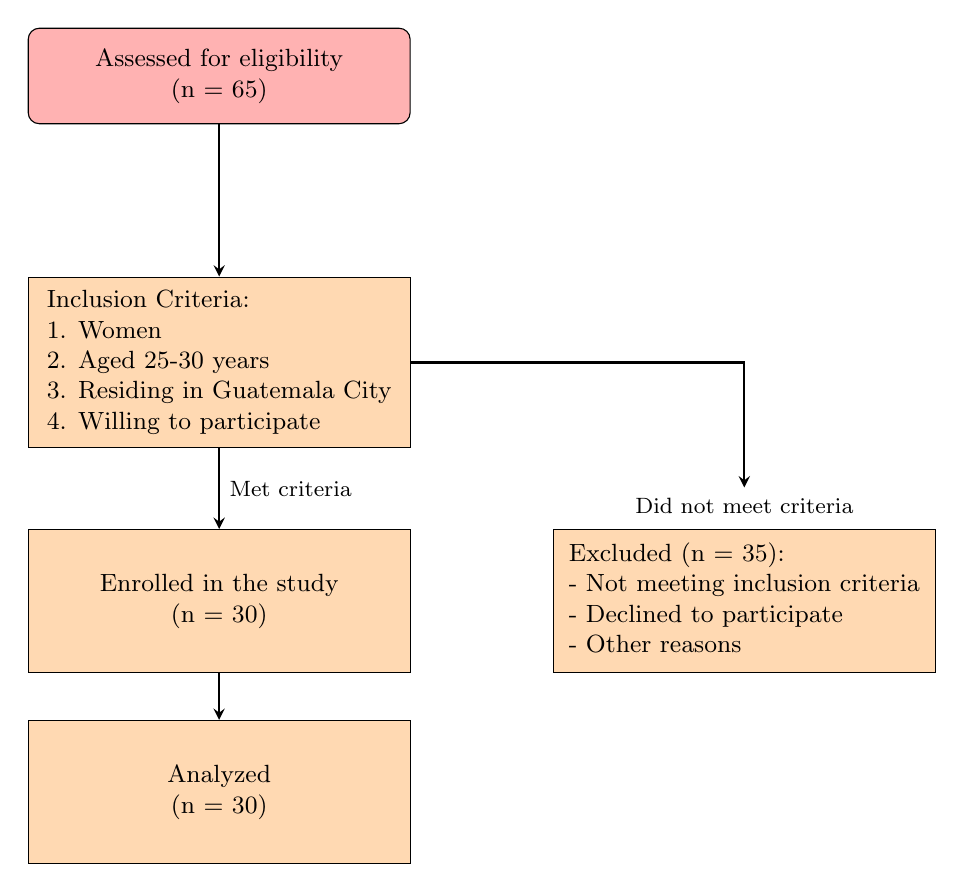
\begin{tikzpicture}[
            node distance=0.1\columnwidth,
            every node/.style={font=\small},
            startstop/.style={rectangle, rounded corners, minimum width=0.4\columnwidth, minimum height=0.1\columnwidth, text centered, draw=black, fill=red!30},
            process/.style={rectangle, minimum width=0.4\columnwidth, minimum height=0.15\columnwidth, text centered, draw=black, fill=orange!30},
            arrow/.style={thick, ->, >=stealth}
        ]
        \node (start) [startstop] {\makecell{Assessed for eligibility\\(n = 65)}};
        \node (criteria) [process, below of=start, yshift=-0.2\columnwidth] {\makecell[l]{Inclusion Criteria:\\1. Women\\2. Aged 25-30 years\\3. Residing in Guatemala City\\4. Willing to participate}};
        \node (enrolled) [process, below of=criteria, yshift=-0.15\columnwidth] {\makecell{Enrolled in the study\\(n = 30)}};
        \node (excluded) [process, right of=enrolled, xshift=0.45\columnwidth] {\makecell[l]{Excluded (n = 35):\\- Not meeting inclusion criteria\\- Declined to participate\\- Other reasons}};
        \node (analyzed) [process, below of=enrolled, yshift=-0.1\columnwidth] {\makecell{Analyzed\\(n = 30)}};
        
        \draw [arrow] (start) -- (criteria);
        \draw [arrow] (criteria) -- node[anchor=west, font=\footnotesize] {Met criteria} (enrolled);
        \draw [arrow] (criteria) -| ([yshift=15pt]excluded.north) node[anchor=north, font=\footnotesize] {Did not meet criteria};
        \draw [arrow] (enrolled) -- (analyzed);
        
        \end{tikzpicture}
    }
    \caption{CONSORT flow diagram of participant selection}
    \label{fig:consort}
\end{figure}



Additionally, the following exclusion criteria were identified: a) Women with chronic illnesses b) Women with autoimmune diseases c) Pregnant women, to avoid any influence of these conditions on the study results. Clarifying these exclusions, participants were warned that if they did not meet the exclusions, the researchers would not be held responsible, as they signed and read the informed consent. This sample and population selection methodology ensured that the research was accurate, relevant, and replicable.

\subsection{Selection and Definition of Variables}\label{selecciuxf3n-y-definiciuxf3n-de-variables}

In this study, variables encompassing psychological and nutritional aspects were selected. Thus integrating both quantitative and qualitative measures to achieve a comprehensive and thorough analysis.\\

\subsubsection{Beck Depression Inventory}
This is an ordinal measure that evaluated the severity of depressive symptoms. The scale is a validated and recommended psychometric tool, and its inclusion allowed for the quantification of the participants' mood in a standardized and reliable manner.

\subsubsection{Dietary Questionnaire}
This is a categorical variable designed to assess the dietary habits of the participants as well as their quality. This questionnaire helped capture detailed information about food consumption and dietary patterns, which was crucial for investigating the relationship between diet and mood.

\section{Hypothesis}\label{hipuxf3tesis}

This study hypothesizes that there is a statistically significant bidirectional relationship between diet and depression, influencing both mood and overall well-being. This hypothesis posits that dietary patterns contribute to mood disturbances, which in turn affect mental and physical health, and that mood disturbances may also influence dietary choices. Confirmation or refutation of this hypothesis will provide insights into the interaction between diet and depression.

\section{Data Collection Procedure}\label{procedimiento-para-recolecciuxf3n-de-datos}

After the topic and methodology for this research were approved, it was necessary to conduct a detailed literature review to validate the importance of the research. It was ensured that the background information was up-to-date and highly reliable.

It was ensured that the matrix instrument was reliable for selecting the searched articles. For this, it was necessary to specify the different inclusion and exclusion criteria. The criteria for article selection were of utmost importance to ensure specificity and clarity. Additionally, research involving young Guatemalan women investigating diet and mood, and finding specific instruments such as scales to measure mood were necessary.

The results of the articles deemed pertinent and necessary for the research were used. Two investigators responsible for this research reviewed the data to minimize bias and extract the most accurate data.

The research data were grouped based on diet and mood scale. A scale was used to measure mood and an interview to analyze the diet of each research participant, using them to understand the relationship between dietary habits and mood.


\subsection{Statistical Analysis and Data Processing}

For this study, we established a significance level ($\alpha$) of 0.05, corresponding to a 95\% confidence interval. This means that p-values less than 0.05 will be considered statistically significant. We chose this conventional level of significance to balance the risks of Type I and Type II errors. The 95\% confidence interval provides a range of values that we can be 95\% certain contains the true population parameter. This approach allows us to make inferences about the population based on our sample data with a known level of confidence.


\subsection{Description and Justification of Methods and Analysis Techniques}\label{descripciuxf3n-y-justificaciuxf3n-de-muxe9todos-y-tuxe9cnicas-de-anuxe1lisis}

The selection of statistical methods and analysis techniques for this study was guided by statistical principles and based on a deep understanding of the nature of the variables involved. Since the goal was to examine possible correlations between variables: dietary habits and mood states, correlation and regression techniques were employed to investigate the relationships between the variables. Correlation allowed us to determine the strength and direction of the relationship between two variables, while regression analysis helped to understand how the variation in the dependent variable was described by the independent variables.\\

Additionally, considering the nature of the data collected, which included ordinal measures (Beck scale) and categorical measures (dietary patterns), methods that fit these characteristics were used. Among them were normality tests to evaluate the distribution of the sample; a crucial step in selecting the most appropriate statistical tests. Furthermore, analysis of variance was used when relevant to compare means between different groups and better understand variations in the variables of interest.\\

This approach not only allowed for establishing the existence of correlations but also exploring the nature and significance of these relationships, providing a solid basis for subsequent interpretations and conclusions.

\subsection{Statistical Procedures}\label{procedimientos-estaduxedsticos}

\subsubsection{Application and Analysis of the Beck Depression Inventory}
After applying the scale to the sample, participants were categorized based on their scores: minimal or no depression, mild depression, moderate, and severe depression. This classification was the central focus for the following analyses.\\

\subsubsection{Normality Tests}
Before proceeding with comparative analyses, as part of the statistical processes, a crucial step was to analyze the normality of the sample. The \emph{Shapiro-Wilk} test implemented in \emph{`SciPy'} was used to check the data distribution. If the sample was normal, the following statistical tests could be performed.\\

\subsubsection{Variance Comparisons (ANOVA)}
An analysis of variance was used to compare dietary patterns among the different depression groups. If significant differences were identified, post-hoc tests were performed to determine where these differences resided.\\

\subsubsection{Correlation and Regression Analysis}
The relationship between the severity of depressive symptoms and dietary habits was explored using Pearson's correlation coefficient and regression analysis. This allowed for a better understanding of the nature and strength of these relationships.

\subsubsection{Data Visualization and Presentation}
With the support of the \emph{`Python'} programming language and \emph{`Jupyter Notebook'} for statistical analysis and Tableau for visualization, the data was presented in a way that highlighted key relationships and important findings, facilitating interpretation.

\subsubsection{Contextualized Interpretation of Results}
All results were interpreted considering reliability and statistical significance. The conclusions were discussed in the context of existing literature and practical implications for the general scientific context and specifically for the Guatemalan population.

\subsection{Inclusion of Key Aspects in the Analysis}\label{inclusiuxf3n-de-aspectos-clave-en-el-anuxe1lisis}

In this research, the integrity and accuracy of statistical analysis were fundamental. Therefore, several key aspects were incorporated to ensure the quality and reliability of the results and conclusions.\\

\subsubsection{Verification of Data Normality}
At each stage of the analysis, normality tests were conducted, such as the Shapiro-Wilk test to assess the distribution of the data where required. This verification was crucial to determine the suitability of selecting statistical tests given the normality of the sample and thus ensure the validity of the proposed interpretations.

\subsubsection{Evaluation of the Reliability of Measurement Tools}
It was essential and fundamental to validate the reliability of the tools used, such as the Beck Depression Inventory and the Dietary Questionnaire. This was done by calculating Cronbach's alpha coefficient, as high reliability ensured that the collected data was consistent and representative.

\subsubsection{Descriptive Statistics of the Sample}
Descriptive statistics of the sample, including means, medians, modes, ranges, and standard deviations, were provided. These statistics offered a clear and understandable view of the data to establish analyses based on a solid foundation for subsequent statistical tests.

\subsubsection{Contextualized Interpretation of Results}
All results were interpreted in light of contextualized hermeneutics based on respective reliability and statistical significance. Clear thresholds for statistical significance were also established, and the findings were discussed in relation to these criteria. This allowed for evaluating the strength and relevance of both the results and the presented conclusions. Additionally, the results were presented based on existing literature and relevant theories in the field. This provided relevant conclusions for the Latin American population, especially Guatemalans.


\section{Ethical Considerations}\label{consideraciones-uxe9ticas}

\subsection{Informed Consent}\label{consentimiento-informado}

Informed consent was obtained from all participants. To achieve this, they were provided with detailed information about the study's objectives, procedures, possible risks, and benefits. Additionally, it was ensured that they understood that their participation was entirely voluntary and that they had the right to withdraw from the study at any time without consequences.

\subsection{Confidentiality and Privacy}\label{confidencialidad-y-privacidad}

Confidentiality and privacy of all collected information were maintained. Participants' personal data were anonymized and kept confidential, ensuring their privacy and protection.

\subsection{Approval by an Ethics Committee}\label{aprobaciuxf3n-de-un-comituxe9-de-uxe9tica}

The research protocol was submitted for review and approval by an ethics committee, ensuring that it met ethical standards and current regulations.

\subsection{Impact and Benefit for Participants and the Community}\label{impacto-y-beneficio-para-los-participantes-y-la-comunidad}

The potential impact and benefits of the research for both the participants and the involved community were evaluated and described. Additionally, emphasis was placed on maximizing benefits and minimizing any potential risks.

\subsection{Budget}\label{presupuesto}

\begin{table}[!ht]
	\centering
	\begin{tabular}{>{\bfseries}l c}
		\toprule
		Item & Cost (Q) \\

		\midrule
		Band-Aids & 30 \\

		Needles & 150 \\

		Cotton & 20 \\

		Alcohol & 20 \\

		Gasoline & 200 \\

		Electricity and Internet & 100 \\

		\midrule
		Total & 520 \\

		\bottomrule
	\end{tabular}
	\caption{Budget for the study}
	\label{tab:presupuesto}
\end{table}

The budget will be covered by the principal investigators.

\subsection{Timeline}\label{cronograma}

\begin{table}[!ht!]
	\centering
	\begin{tabular}{@{}ll@{}}
		\toprule
		\textbf{Item}                & \textbf{Detail}     \\ \midrule
		Start Date              & February 2024         \\
		End Date        & June 2024           \\
		Duration                     & 5 months              \\ \bottomrule
	\end{tabular}
	\caption{Study Dates and Duration}
	\label{tab:fechas-duracion}
\end{table}

\section{Results}\label{resultados}

\subsection{Sociodemographic Data}

\begin{figure}[!ht]
	\centering
	\includegraphicsmax{freq.age.pdf}
	\caption{Age Frequency}
	\label{fig:Figure1}
\end{figure}

\begin{table}[!ht]
	\centering
	\resizebox{0.8\columnwidth}{!}{
		\begin{tabular}{@{}rrrr@{}}
			\toprule
			\textbf{Statistic}             & \textbf{Total Beck} & \textbf{Total Diet}  \\ \midrule
			\textbf{N}                       & 30.00                  & 30.00                   \\
			\textbf{Mean}                   & 19.00                  & 4.77                    \\
			\textbf{Median}                 & 17.00                  & 6.00                    \\
			\textbf{Standard Deviation}     & 9.28                   & 9.58                    \\
			\textbf{Minimum}                  & 7.00                   & -17.00                  \\
			\textbf{Maximum}                  & 42.00                  & 21.00                   \\
			\textbf{Skewness}               & 0.97                   & -0.22                   \\
			\textbf{Kurtosis}                & 0.14                   & -0.60                   \\
			\textbf{Shapiro-Wilk W}       & 0.90                   & 0.97                    \\
			\textbf{Shapiro-Wilk p-value} & 0.01                   & 0.63                    \\ \bottomrule
		\end{tabular}
	}

	\caption{Descriptive statistics of the variables}

	\label{tab:descriptives}
\end{table}

\subsubsection{Total Beck Scale}
The score on the Beck scale shows a non-normal distribution with a right skew. This suggests that there are more individuals with lower depression scores, but with a wide variability. The high standard deviation indicates significant differences between individual scores.

\subsubsection{Total Diet Questionnaire}
The distribution of diet scores is normal and has negative values, which are allowed by the questionnaire. The median is higher than the mean, indicating a slight tendency towards higher values.


\begin{figure}[!ht]
	\centering
	\begin{subfigure}[b]{\subfigwidth}
		\centering
		\includegraphics[width=\linewidth]{Box_Plot_of_dieta_total.pdf}
		\caption{Total Diet}
		\label{fig:BoxPlotDietaTotal}
	\end{subfigure}
	\hspace{0.5em}
	\begin{subfigure}[b]{\subfigwidth}
		\centering
		\includegraphics[width=\linewidth]{Box_Plot_of_beck_total.pdf}
		\caption{Beck Total}
		\label{fig:BoxPlotBeckTotal}
	\end{subfigure}

	\caption{Box and Whisker Plots of Variables}
	\label{fig:BoxPlots}
\end{figure}

\begin{table}[H]
   \centering
   \resizebox{\textwidth}{!}{%
   \begin{tabular}{@{}llll@{}}
       \toprule
       \textbf{Variable 1}         & \textbf{Variable 2}         & \textbf{$R^2$}     & \textbf{P Value} \\ \midrule
       fruit consumption           & loss of pleasure            & -0.488897          & 0.006            \\
       fruit consumption           & suicidal thoughts           & -0.480279          & 0.007            \\
       sugar consumption           & pessimism                   & 0.432226           & 0.017            \\
       soda consumption            & loss of interest            & 0.418097           & 0.021            \\
       flour consumption           & concentration difficulty    & 0.413595           & 0.023            \\
       red meat consumption        & pessimism                   & 0.407187           & 0.026            \\
       ginger consumption          & agitation                   & -0.403648          & 0.027            \\
       fruit consumption           & punishment feeling          & -0.397679          & 0.030            \\
       fruit consumption           & dissatisfaction             & -0.390977          & 0.033            \\
       red meat consumption        & irritability                & 0.388368           & 0.034            \\
       sugar consumption           & irritability                & 0.377928           & 0.039            \\
       flour consumption           & loss of interest            & 0.377707           & 0.040            \\
       total diet questionnaire    & irritability                & -0.372452          & 0.043            \\
       soda consumption            & indecision                  & 0.371774           & 0.043            \\
       alcohol consumption         & agitation                   & 0.365651           & 0.047            \\
       fruit consumption           & loss of interest            & -0.365214          & 0.047            \\
       soda consumption            & appetite changes            & 0.353747           & 0.055            \\
       total diet questionnaire    & punishment feeling          & -0.351071          & 0.057            \\ \bottomrule
   \end{tabular}
   } % resizebox
   \caption{Correlation Table}
   \label{tab:tableOfCorr}
\end{table}





The table \ref{tab:tableOfCorr} shows the correlations between various consumption variables and different emotional or psychological symptoms, along with the associated p-values indicating the statistical significance of these correlations.

There is a significant negative correlation between fruit consumption and loss of pleasure, suggesting that higher fruit consumption is associated with a lower loss of pleasure. There is also a significant negative correlation between fruit consumption and suicidal thoughts, indicating that higher fruit consumption is associated with a lower frequency of suicidal thoughts.

Other observed correlations include a positive correlation between sugar consumption and pessimism, suggesting that higher sugar consumption is associated with higher levels of pessimism. A positive correlation between soda consumption and loss of interest indicates that higher soda consumption is associated with greater loss of interest.

Additionally, there is a positive correlation between flour consumption and difficulty concentrating, suggesting that higher flour consumption is associated with greater difficulty concentrating. There is also a positive correlation between red meat consumption and pessimism, indicating that higher red meat consumption is associated with higher levels of pessimism.

There is a significant negative correlation between fruit consumption and feelings of punishment, indicating that higher fruit consumption is associated with lower feelings of punishment. There is also a negative correlation between fruit consumption and dissatisfaction, suggesting that higher fruit consumption is associated with lower levels of dissatisfaction.

A positive correlation was observed between red meat consumption and irritability, indicating that higher red meat consumption is associated with greater irritability.

Most of the negative correlations involve fruit consumption, which could suggest a protective effect of fruit consumption against certain negative psychological symptoms. The positive correlations between sugar and soda consumption with negative symptoms such as pessimism and loss of interest could indicate the need to moderate the consumption of these products to improve emotional well-being.

All mentioned correlations are significant with a p-value \textless{} 0.05, which supports the robustness of these associations. These insights can be used to recommend dietary adjustments as part of a holistic approach to improving emotional and mental well-being.

Cronbach's $\alpha$ is a measure of the internal consistency of a scale. Values between 0.7 and 0.8 are generally considered acceptable, suggesting that the scale has adequate reliability. In this case, a value of 0.741 indicates that the items in the diet questionnaire are reasonably correlated and measure the same underlying construct.

McDonald's $\omega$ is another measure of internal consistency and is often considered a more accurate estimate than Cronbach's $\alpha$. A value above 0.9 is considered excellent, indicating high reliability of the scale. In this case, a value of 0.904 suggests that the questionnaire is very reliable and that the items are consistent in measuring the construct.

Both values indicate good internal consistency, although McDonald's $\omega$ is notably higher than Cronbach's $\alpha$. This can occur when the items have different factor loadings, and McDonald's $\omega$, which takes these differences into account, provides a more accurate estimate of reliability. The diet questionnaire we developed is reliable for use in research and practical applications, as both reliability metrics exceed the generally accepted thresholds.


\subsection{Beck Depressive Symptoms}
\begin{figure}[!ht]
	\centering
	\includegraphicsmax{sintomasDepresivosBeckGraph.pdf}
	\caption{Heat Map: Depressive Symptoms}
	\label{fig:Figure2}
\end{figure}
\vspace{-1em} % Adjust vertical space

\subsection{Dietary Habits of Young Guatemalan Women}
\begin{figure}[!ht]
	\centering
	\includegraphicsmax{dietGraph.pdf}
	\caption{Heat Map: Dietary Questionnaire}
	\label{fig:Figure3}
\end{figure}

\section{Discussion of Results}\label{discusiuxf3n-de-resultados}

This study aimed to analyze the relationship between dietary habits and the severity of depressive symptoms in young Guatemalan women. The results provide significant evidence of these interactions and offer valuable insights into understanding the relationship between diet and depression in this specific population.

\subsection{Summary of Main Findings}\label{resumen-de-hallazgos-principales}

Our study revealed significant correlations between certain dietary patterns and specific depressive symptoms. In particular, a strong negative association was found between fruit consumption and various depressive symptoms, including loss of pleasure $(r = -0.49, p = 0.006)$ and suicidal thoughts $(r = -0.48, p = 0.007)$. On the other hand, positive correlations were observed between the consumption of processed foods (such as sugars, sodas, and flours) and symptoms such as pessimism, loss of interest, and difficulty concentrating.\\

\subsection{Interpretation of Results}\label{interpretaciuxf3n-de-resultados}

\subsubsection{Protective Effect of Fruit Consumption}

The negative correlation between fruit consumption and depressive symptoms suggests a possible protective effect of a fruit-rich diet against depression. This could be attributed to the nutrients and antioxidants present in fruits, which may have a positive impact on mental health. The particularly strong association with the reduction of suicidal thoughts is a notable finding that warrants further investigation.\\

This relationship could be explained by several mechanisms:

\begin{enumerate}
	\item Antioxidants present in fruits may reduce oxidative stress, which has been associated with depression.\\

	\item Fruits are rich in essential vitamins and minerals for optimal neurological functioning.\\

	\item The dietary fiber in fruits may positively influence the gut microbiota, which in turn affects the gut-brain axis.
\end{enumerate}

\subsubsection{Negative Impact of Processed Foods}\label{impacto-negativo-de-alimentos-procesados}

The positive correlations between the consumption of processed foods and depressive symptoms support the hypothesis that a diet high in refined sugars and saturated fats may contribute to the development or exacerbation of depressive symptoms. Possible mechanisms for this relationship include:

\begin{enumerate}
	\item Processed foods can cause blood glucose spikes, which can affect mood.
	\item These foods often lack essential nutrients for mental health.
	\item Excessive consumption of processed foods can lead to obesity, which has been associated with a higher risk of depression.
\end{enumerate}



\subsection{Comparison with Existing Literature}\label{comparaciuxf3n-con-literatura-existente}

Our findings on the protective effect of fruits are consistent with previous studies that have found associations between fruit and vegetable consumption and a reduced risk of depression. For example, a meta-analysis conducted by \parencite{liuFruitVegetableConsumption2016} found that higher fruit and vegetable consumption was associated with a lower risk of depression. However, our study provides specific evidence of the relationship between fruit consumption and specific depressive symptoms in a little-studied population: young Guatemalan women.\\

The positive association between processed foods and depressive symptoms also aligns with previous research linking Western diets (high in processed foods) with a higher risk of depression. For example, \parencite{laneUltraProcessedFoodConsumption2022} found that a diet characterized by processed foods was associated with a higher likelihood of depression and anxiety in women. Nonetheless, our study provides a more detailed view by examining correlations with specific symptoms. Additionally, several other studies have been published evaluating the relationship between ultra-processed food consumption and depression, as well as other mental disorders. Our study included a total of 17 observational studies (n = 385,541); 15 cross-sectional and 2 prospective. Higher consumption of ultra-processed foods was cross-sectionally associated with greater odds of depressive and anxiety symptoms, both when these outcomes were evaluated together (odds ratio of common mental disorder symptoms: 1.53, 95\% CI 1.43 to 1.63) and separately (odds ratio of depressive symptoms: 1.44, 95\% CI 1.14 to 1.82; and, odds ratio of anxiety symptoms: 1.48, 95\% CI 1.37 to 1.59). Additionally, a meta-analysis of prospective studies showed that greater intake of ultra-processed foods was associated with an increased risk of subsequent depression (hazard ratio: 1.22, 95\% CI 1.16 to 1.28). Although we found evidence of associations between ultra-processed food consumption and adverse mental health, rigorously designed prospective and experimental studies are needed to better understand the causal pathways.

\subsection{Implications}\label{implicaciones}

These results have important implications for both clinical practice and public health:

\begin{enumerate}
	\item Dietary interventions: The findings suggest that dietary interventions, particularly increasing fruit consumption and reducing processed foods, could be effective strategies for the prevention and management of depression in young women.
	\item Public health policies: These results could inform public health policies aimed at improving mental health through the promotion of healthy diets. For example, nutritional education programs focused on increasing fruit consumption and reducing the intake of processed foods could be implemented.
	\item Integrated approach: The association between diet and depressive symptoms reinforces the importance of an integrated approach to depression treatment that considers both psychological and nutritional factors. Mental health professionals might consider including dietary recommendations as part of their treatment plans.
	\item Prevention: Since our study focused on young women, the results suggest that early dietary interventions could play an important role in preventing depression in this population.
\end{enumerate}

\section{Limitations}\label{limitaciones}

It is important to acknowledge the limitations of this study:

\begin{enumerate}
	\item Sample size: With 30 participants, the sample size is relatively small, which may limit the generalizability of the results. Future studies should consider larger samples to increase statistical power.
	\item Cross-sectional design: The cross-sectional design of the study does not allow for establishing causal relationships between diet and depressive symptoms. Longitudinal studies are needed to determine the direction of causality.
	\item Specific population: The study focused on young Guatemalan women, which may limit the applicability of the results to other populations. Studies in different demographic groups are needed to confirm whether these findings are generalizable.
	\item Definition of dietary patterns: As observed in the literature, the lack of a standardized definition of ``healthy diet'' can make comparison between studies difficult. In our case, we focused on specific foods rather than general dietary patterns, which may limit comparability with other studies.
	\item Variability in depression measurement: Although we used the Beck scale, which is widely validated, the literature notes that variability in depression measures across studies can make it difficult to compare results.
	\item Confounding factors: Although several demographic and lifestyle factors were controlled for, there may be other unmeasured confounding factors that could influence the relationship between diet and depression.
\end{enumerate}


\section{Recommendations for Future Research}\label{recomendaciones-para-futuras-investigaciones}

Based on our findings and limitations, we recommend:
\begin{enumerate}
	\item Conduct longitudinal studies to establish causal relationships between dietary patterns and depressive symptoms.
	\item Investigate the biological mechanisms underlying the relationship between fruit consumption and the reduction of depressive symptoms.
	\item Explore the effectiveness of specific dietary interventions in the prevention and treatment of depression.
	\item Expand the study to more diverse and larger populations.
	\item Standardize the definition and measurement of dietary patterns to facilitate comparison between studies.
	\item Use multiple measures of depression, including structured clinical interviews, to obtain a more comprehensive assessment of depressive symptoms.
	\item Investigate the interaction between diet and other lifestyle factors, such as exercise and sleep, in relation to depression.
\end{enumerate}

\section{Conclusion}\label{conclusiuxf3n}

This study provides important evidence on the relationship between dietary patterns and depressive symptoms in young Guatemalan women. The findings underscore the potential protective role of a fruit-rich diet and the possible negative effects of processed foods on mental health. Although more research is needed, these results suggest that dietary interventions could be a valuable component in prevention and treatment strategies for depression.\\

The complexity of the relationship between diet and depression evidenced in this study underscores the need for a multidisciplinary approach to depression research and treatment. As we advance in understanding these interactions, it is crucial that mental health professionals, nutritionists, and public health policymakers work together to develop comprehensive strategies that address both the nutritional and psychological aspects of mental health.

%\nocite{*}





\printbibliography

\end{document}


%
%%%
%%% Copyright (C) 2019 by Daniel A. Weiss <daniel.weiss.led at gmail.com>
%%%
%%% This work may be distributed and/or modified under the
%%% conditions of the LaTeX Project Public License (LPPL), either
%%% version 1.3c of this license or (at your option) any later
%%% version.  The latest version of this license is in the file:
%%%
%%% http://www.latex-project.org/lppl.txt
%%%
%%% Users may freely modify these files without permission, as long as the
%%% copyright line and this statement are maintained intact.
%%%
%%% This work is not endorsed by, affiliated with, or probably even known
%%% by, the American Psychological Association.
%%%
%%% This work is "maintained" (as per LPPL maintenance status) by
%%% Daniel A. Weiss.
%%%
%%% This work consists of the file  apa7.dtx
%%% and the derived files           apa7.ins,
%%%                                 apa7.cls,
%%%                                 apa7.pdf,
%%%                                 README,
%%%                                 APA7american.txt,
%%%                                 APA7british.txt,
%%%                                 APA7dutch.txt,
%%%                                 APA7english.txt,
%%%                                 APA7german.txt,
%%%                                 APA7ngerman.txt,
%%%                                 APA7greek.txt,
%%%                                 APA7czech.txt,
%%%                                 APA7turkish.txt,
%%%                                 APA7endfloat.cfg,
%%%                                 Figure1.pdf,
%%%                                 shortsample.tex,
%%%                                 longsample.tex, and
%%%                                 bibliography.bib.
%%%
%%%
%%% End of file `./samples/longsample.tex'.